\documentclass[11pt]{article}
\usepackage[margin=1in]{geometry}
\usepackage[T1]{fontenc}
\usepackage{lmodern}
\usepackage{xcolor}
\usepackage{hyperref}
\usepackage{amsmath,amssymb,amsthm}
\usepackage{booktabs}
\usepackage{graphicx}
\usepackage{caption}

\definecolor{gcblue}{HTML}{005DAB}
\definecolor{gcorange}{HTML}{FE5000}
\definecolor{muted}{HTML}{586F82}
\hypersetup{colorlinks=true, linkcolor=gcblue, citecolor=gcblue, urlcolor=gcblue}

\newtheorem{definition}{Definition}
\newtheorem{proposition}{Proposition}
\newtheorem{remark}{Remark}
\newcommand{\E}{\mathbb{E}}
\newcommand{\Prb}{\mathbb{P}}

\title{\textbf{LLMs Can Play (Global) Games}\\[0.3em]
\large Lecture Notes on Natural-Language Coordination, Validation, and Extensions}
\author{Khaled Eltokhy\\CUNY Graduate Center, Department of Economics}
\date{May 2026}

\begin{document}
\maketitle

\begin{abstract}
These notes develop the logic behind a canonical global game and explain how large language model (LLM) agents can be used as controlled subjects in a natural-language version of that environment. The target reader is a first-year PhD student in economics who has seen static Bayesian games and basic equilibrium reasoning, but may not yet have worked through Morris--Shin global games. The central idea is simple: in a coordination game, a citizen wants to join a risky collective action only if enough others also join. A latent fundamental determines how hard coordination is, and each agent observes only a noisy private signal about that fundamental. The canonical Morris--Shin result is that small private-signal noise selects a unique monotone threshold equilibrium. This gives a sharp empirical prediction: aggregate joining decreases as the regime becomes stronger. The LLM experiment embeds the private signal in prose rather than numbers and asks whether LLM actions reproduce the same comparative static. Communication and monitoring are then natural extensions of the same laboratory.
\end{abstract}

\tableofcontents

\section{The economic question}

Many political and economic actions are strategic complements. Joining a protest, attacking a currency peg, withdrawing from a bank, adopting a technology, or participating in a platform all become more attractive when enough others do the same. This creates a coordination problem. If everyone expects participation, participation can be optimal. If everyone expects nonparticipation, nonparticipation can also be optimal.

Global games, introduced by Carlsson and van Damme (1993) and developed by Morris and Shin (2003), study how small amounts of private information discipline this multiplicity. Agents do not observe the true state of the world directly. Instead, each receives a noisy signal. The central result is that private information can select a unique threshold equilibrium.

The experiment in the slides asks whether LLM agents can play this canonical structure when the signal is embedded in natural language. The title claim, \emph{LLMs Can Play (Global) Games}, is deliberately about validation first. If LLM agents do not reproduce the canonical comparative static, the later communication and monitoring exercises are not credible. If they do, the same environment becomes a laboratory for richer coordination questions.

\section{The canonical coordination problem}

Consider a continuum of citizens indexed by $i\in[0,1]$. Each citizen chooses
\[
  a_i\in\{0,1\},
\]
where $a_i=1$ means \emph{join} and $a_i=0$ means \emph{stay}. Let
\[
  A=\int_0^1 a_i\,di
\]
denote the aggregate mass of citizens who join.

There is a latent fundamental $\theta$, interpreted here as regime strength. A lower value of $\theta$ means the regime is easier to topple; a higher value means it is stronger. The collective action succeeds if the mass of citizens who join is at least as large as regime strength:
\[
  \text{success} \iff A\ge \theta.
\]
For example, if $\theta=0.7$, at least 70 percent of citizens must join for the regime to collapse.

Payoffs are normalized in the simplest way. Joining costs $c$, where $0<c<1$. If the regime collapses, joining gives benefit $1$ and cost $c$, so the net payoff is $1-c$. If the regime does not collapse, joining gives no benefit but still costs $c$:
\[
  u(1)=
  \begin{cases}
  1-c, & \text{if collapse occurs},\\
  -c, & \text{if collapse does not occur}.
  \end{cases}
\]
The payoff from not joining is normalized to zero:
\[
  u(0)=0.
\]
Thus an agent joins if and only if the posterior probability of collapse is high enough:
\[
  \Prb(\text{collapse}\mid\text{information})\ge c.
\]
This is the whole decision rule. Joining is optimal when the probability of success is large enough to justify the cost.

The core tension is therefore:
\begin{quote}
A citizen wants to join only when she expects enough others to join.
\end{quote}
This is the source of strategic complementarity. My incentive to join depends on my belief about aggregate participation, and that aggregate participation depends on the beliefs and actions of others.

\section{Information: what agents know}

The regime strength $\theta$ is not observed directly. Each citizen receives a noisy private signal
\[
  x_i=\theta+\sigma\varepsilon_i,
  \qquad
  \varepsilon_i\sim\mathcal{N}(0,1),
\]
where $\sigma>0$ measures signal noise. A low signal is good news for the uprising: it suggests the regime is weak. A high signal is bad news: it suggests the regime is strong.

In the standard Morris--Shin benchmark, agents share a common prior over $\theta$; often the derivation is presented using a diffuse or improper uniform prior to keep the posterior algebra transparent. The essential logic does not require the audience to memorize that prior. The key objects are:
\begin{itemize}
  \item a latent fundamental $\theta$;
  \item private signals $x_i$ that are informative but noisy;
  \item a coordination payoff in which joining is attractive only if enough others join.
\end{itemize}

\section{Complete information and multiplicity}

Before adding private noise, it is useful to see the multiplicity problem. Suppose everyone observes $\theta$.

If everyone joins, then $A=1$. Collapse occurs whenever $1\ge \theta$. Hence for any $\theta<1$, ``everyone joins'' can be an equilibrium: each agent expects enough others to join, so joining has success probability one and payoff $1-c>0$.

If nobody joins, then $A=0$. Collapse does not occur whenever $0<\theta$. Hence for any $\theta>0$, ``nobody joins'' can also be an equilibrium: each agent expects failure, so joining has payoff $-c<0$.

Therefore, for
\[
  0<\theta<1,
\]
there are two self-confirming equilibria:
\[
  A=1
  \qquad\text{and}\qquad
  A=0.
\]
Everyone joining is self-confirming. Nobody joining is also self-confirming. This is the equilibrium-selection problem that global games resolve.

\section{Canonical result: threshold behavior}

The canonical Morris--Shin result is that the Bayesian Nash equilibrium is monotone in the private signal. There is a cutoff $x^*$ such that
\[
  \text{join} \iff x_i\le x^*.
\]
This threshold rule is the main theoretical benchmark. The experiment asks whether agents who receive natural-language versions of $x_i$ behave as the canonical model predicts.

Why is a cutoff natural? Lower signals indicate a weaker regime. A citizen with a lower signal believes success is more likely. She also understands that other citizens' signals are centered around the same underlying fundamental, so a low signal is informative about the distribution of others' likely signals and actions. Thus the incentive to join is stronger after lower signals. Under standard single-crossing and monotonicity arguments, this leads to a threshold strategy.

The cutoff $x^*$ is pinned down by the marginal type: the citizen with signal exactly $x^*$ must be indifferent between joining and staying. Types below the cutoff strictly prefer to join; types above it strictly prefer to stay.

\begin{proposition}[Canonical global-game prediction]
In the Morris--Shin regime-change environment with noisy private signals, equilibrium behavior is characterized by a threshold rule. Aggregate participation is decreasing in the regime-strength fundamental $\theta$.
\end{proposition}

The statement uses the normalized regime-change convention in which $A\in[0,1]$ is the mass of attackers and $\theta$ is the participation threshold required for success. Thus the boundary condition $A(\theta^*)=\theta^*$ means that, at $\theta^*$, the mass attacking exactly equals the regime strength that must be exceeded.

\section{Deriving the threshold prediction}

This section derives the key prediction at the level needed for a first-year PhD student. The derivation has four steps: guess a cutoff strategy, compute aggregate participation, define the collapse threshold, and impose indifference for the marginal agent.

\subsection{Step 1: Guess a monotone cutoff strategy}

Because lower $x_i$ means the regime appears weaker, look for a monotone equilibrium in which citizens join when their signal is sufficiently low:
\[
  a_i(x_i)=
  \begin{cases}
  1, & x_i\le x^*,\\
  0, & x_i>x^*.
  \end{cases}
\]
The unknown object is the attack threshold $x^*$. If an agent's signal is bad enough, she joins.

\subsection{Step 2: Aggregate participation under the cutoff}

Fix a true regime strength $\theta$. Citizens join when $x_i\le x^*$. Since
\[
  x_i=\theta+\sigma\varepsilon_i,
  \qquad \varepsilon_i\sim\mathcal{N}(0,1),
\]
this condition is
\begin{align*}
  \theta+\sigma\varepsilon_i&\le x^*,\\
  \varepsilon_i&\le \frac{x^*-\theta}{\sigma}.
\end{align*}
Therefore the fraction of agents who join is
\[
  A(\theta)=\Phi\left(\frac{x^* - \theta}{\sigma}\right),
\]
where $\Phi$ is the standard normal CDF. This expression already shows why the global-game prediction is downward-sloping: a stronger regime shifts signals upward, so fewer agents fall below the attack threshold.

\subsection{Step 3: The collapse threshold $\theta^*$}

The regime collapses when
\[
  A(\theta)\ge \theta.
\]
Substituting the expression for aggregate participation gives
\[
  \Phi\left(\frac{x^*-\theta}{\sigma}\right)\ge \theta.
\]
There is a critical value $\theta^*$ at which the regime is exactly on the boundary between collapse and survival:
\[
  \Phi\left(\frac{x^*-\theta^*}{\sigma}\right)=\theta^*.
\]
For $\theta<\theta^*$, the regime collapses. For $\theta>\theta^*$, it survives.

\subsection{Step 4: The marginal agent's indifference condition}

Now consider the marginal agent who observes exactly $x^*$. This agent must be indifferent between joining and staying. Since joining gives payoff $1-c$ if collapse occurs and $-c$ otherwise, expected payoff from joining is
\begin{align*}
  \Prb(\text{collapse}\mid x^*)(1-c)
  +\left[1-\Prb(\text{collapse}\mid x^*)\right](-c).
\end{align*}
This simplifies to
\[
  \Prb(\text{collapse}\mid x^*)-c.
\]
Staying gives zero, so indifference requires
\[
  \Prb(\text{collapse}\mid x_i=x^*)=c.
\]
Since collapse occurs when $\theta\le \theta^*$, this is
\[
  \Prb(\theta\le \theta^*\mid x_i=x^*)=c.
\]
This is the second key equation. The first equation says the regime is just barely collapsing at $\theta^*$. The second says the marginal attacker is just barely willing to attack at $x^*$.

Under the diffuse-prior Morris--Shin benchmark and normal noise, the posterior is
\[
  \theta\mid x_i\sim\mathcal{N}(x_i,\sigma^2).
\]
Thus for the marginal agent observing $x^*$,
\[
  \Prb(\theta\le \theta^*\mid x_i=x^*)
  =\Phi\left(\frac{\theta^*-x^*}{\sigma}\right).
\]
The indifference condition becomes
\[
  \Phi\left(\frac{\theta^*-x^*}{\sigma}\right)=c.
\]
Apply $\Phi^{-1}$ and rearrange:
\begin{align*}
  \frac{\theta^*-x^*}{\sigma}&=\Phi^{-1}(c),\\
  x^*&=\theta^*-\sigma\Phi^{-1}(c).
\end{align*}
Now plug this into the collapse-threshold equation:
\begin{align*}
  \theta^*
  &=\Phi\left(\frac{x^*-\theta^*}{\sigma}\right)\\
  &=\Phi\left(\frac{\theta^*-\sigma\Phi^{-1}(c)-\theta^*}{\sigma}\right)\\
  &=\Phi\left(-\Phi^{-1}(c)\right)\\
  &=1-c.
\end{align*}
Hence the clean solution in this normalized version is
\[
  \theta^*=1-c,
  \qquad
  x^*=1-c-\sigma\Phi^{-1}(c).
\]
The regime collapses if $\theta\le 1-c$ and survives if $\theta>1-c$. Each agent joins if
\[
  x_i\le 1-c-\sigma\Phi^{-1}(c).
\]

The interpretation is immediate. If attacking is cheap, $c$ is low and $1-c$ is high, so the regime can collapse even when it is relatively strong. If attacking is expensive, $c$ is high and $1-c$ is low, so collapse occurs only when fundamentals are very weak. Private noise selects one equilibrium by turning the coordination problem into a threshold problem.

\section{From the threshold rule to a testable prediction}

The solved model implies
\[
  A(\theta)=\Phi\left(\frac{x^* - \theta}{\sigma}\right).
\]
This equation is the bridge from theory to the experiment. The researcher does not need to recover each agent's full posterior beliefs. The key validation target is the comparative static:
\[
  \frac{dA(\theta)}{d\theta}
  =-\frac{1}{\sigma}\phi\left(\frac{x^*-\theta}{\sigma}\right)<0,
\]
where $\phi$ is the standard normal density. Equivalently,
\[
  \theta \uparrow \quad \Rightarrow \quad A(\theta) \downarrow.
\]
As regime strength rises, joining should fall in a smooth, normal-CDF-shaped way. In the experiment, this becomes an observable validation exercise: assign values of $\theta$, generate private signals and prose briefings from those values, ask LLM agents whether to join, and test whether the join rate declines with the assigned latent fundamental.

\begin{figure}[h]
  \centering
  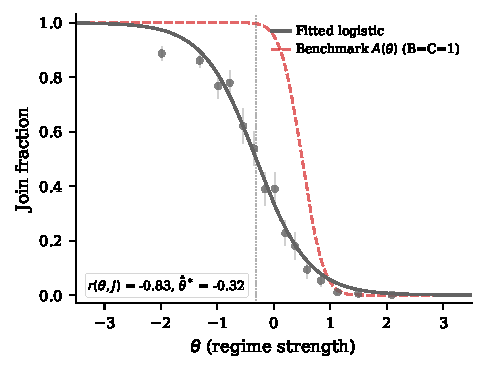
\includegraphics[width=0.78\textwidth]{../paper/figures/fig01_sigmoid.pdf}
  \caption{Baseline validation: LLM join rates decline as the latent regime-strength fundamental increases.}
\end{figure}

\section{Why use LLM agents?}

The methodological idea is related to Horton (2023), who proposes using LLMs as simulated economic agents. The present design uses LLM agents not because they are literal citizens, but because they provide experimental control in a language-rich environment.

LLM calls have several useful properties:
\begin{itemize}
  \item \textbf{Statelessness.} A call has no memory unless the researcher supplies it.
  \item \textbf{Natural language.} The information environment can be prose rather than a numeric table.
  \item \textbf{Known latent state.} The researcher knows $\theta$, $x_i$, and treatment assignment.
  \item \textbf{Prompt manipulation.} Counterfactual information structures can be implemented cleanly.
  \item \textbf{Scale.} Many agents, signals, and treatments can be run cheaply.
\end{itemize}

The validation exercise is therefore not a claim that LLMs are representative humans. It is a claim that LLMs can act as controlled agents in a canonical strategic environment whose theoretical benchmark is known.

\section{Embedding the private signal in prose}

The experiment maps the numeric private signal $x_i$ into a natural-language briefing. The LLM does not see the true value of $\theta$ or the numerical signal. It sees prose such as:
\begin{quote}
\textbf{Private briefing.} The regime's cohesion is visibly fraying. Street talk has shifted from complaint to anticipation. Security forces show friction and delays.
\end{quote}
The econometrician, however, knows the latent value that generated the briefing. This is the key measurement advantage. The LLM sees language; the researcher knows the hidden state and the comparative static implied by the theory.

\section{Validation: not just generic sentiment}

A natural concern is that LLMs may merely react to generic positive or negative sentiment in the text. The validation design therefore includes falsification treatments.

\begin{itemize}
  \item \textbf{Pure.} The prose signal is intact. The threshold relationship should appear.
  \item \textbf{Scramble.} The mapping between latent signal and prose is destroyed. The relationship should collapse.
  \item \textbf{Flip.} The signal content is reversed. The relationship should flip.
\end{itemize}

\begin{figure}[h]
  \centering
  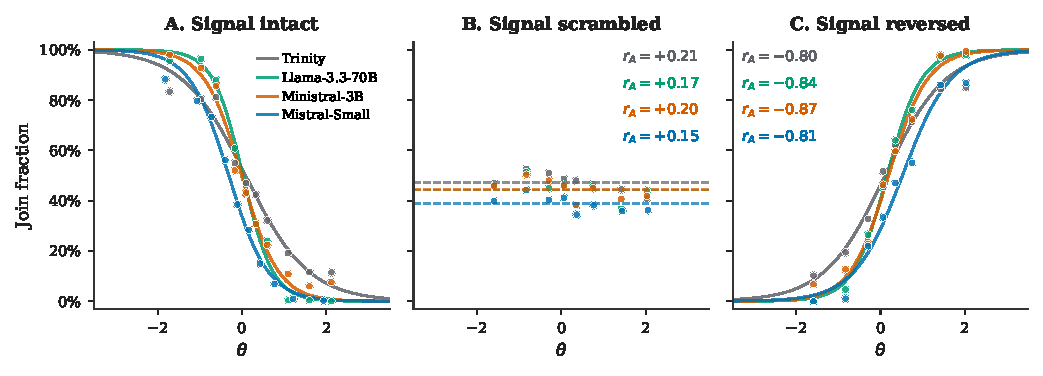
\includegraphics[width=0.95\textwidth]{../paper/figures/fig03_falsification.pdf}
  \caption{Falsification tests: the signal-to-action relationship appears in the pure condition, collapses when the assignment is scrambled, and reverses when signal content is flipped.}
\end{figure}

These tests matter because they ask whether LLM behavior tracks the latent strategic signal rather than surface affect. For the purpose of the title claim, this is the central evidence that LLMs can play the canonical global game.

\section{Extensions: communication and monitoring}

Once the baseline is validated, the environment can be extended. The first extension allows citizens to send short messages to neighbors before choosing whether to join. In a global game, communication can transform private information into social information. A citizen's message is informative not only about that citizen's signal but also about likely aggregate behavior.

The second extension monitors the communication channel. A warning is added to the messaging prompt, but the final decision prompt is unchanged. Because calls are stateless, changes in final actions must operate through changed message content in the main design. Monitoring therefore becomes a stress test for coordination through language.

The key mechanism result is that monitoring lowers participation more than it changes stated beliefs about others' participation. One interpretation is that monitored speech becomes less informative or more cautious, degrading the peer-information channel even when reported beliefs do not collapse.

\section{What a first-year PhD student should take away}

There are four main lessons.

\begin{enumerate}
  \item \textbf{Global games solve a coordination problem by adding private information.} Noisy signals turn multiple-equilibrium intuition into a unique threshold prediction.
  \item \textbf{The empirical object is a comparative static.} The key prediction is not a single action but a declining join-rate curve in regime strength.
  \item \textbf{LLMs are useful here because the benchmark is sharp.} The theory tells us what should happen if agents understand the strategic environment.
  \item \textbf{Communication and monitoring are extensions.} They use the validated laboratory to study richer information structures, not to replace the canonical result.
\end{enumerate}

\section*{References}

\begin{itemize}
  \item Carlsson, Hans, and Eric van Damme. 1993. ``Global Games and Equilibrium Selection.'' \emph{Econometrica} 61(5): 989--1018.
  \item Horton, John J. 2023. ``Large Language Models as Simulated Economic Agents: What Can We Learn from Homo Silicus?'' NBER Working Paper 31122.
  \item Morris, Stephen, and Hyun Song Shin. 2003. ``Global Games: Theory and Applications.'' In \emph{Advances in Economics and Econometrics}.
\end{itemize}

\end{document}
